% Options for packages loaded elsewhere
\PassOptionsToPackage{unicode}{hyperref}
\PassOptionsToPackage{hyphens}{url}
%
\documentclass[
]{article}
\usepackage{lmodern}
\usepackage{amsmath}
\usepackage{ifxetex,ifluatex}
\ifnum 0\ifxetex 1\fi\ifluatex 1\fi=0 % if pdftex
  \usepackage[T1]{fontenc}
  \usepackage[utf8]{inputenc}
  \usepackage{textcomp} % provide euro and other symbols
  \usepackage{amssymb}
\else % if luatex or xetex
  \usepackage{unicode-math}
  \defaultfontfeatures{Scale=MatchLowercase}
  \defaultfontfeatures[\rmfamily]{Ligatures=TeX,Scale=1}
\fi
% Use upquote if available, for straight quotes in verbatim environments
\IfFileExists{upquote.sty}{\usepackage{upquote}}{}
\IfFileExists{microtype.sty}{% use microtype if available
  \usepackage[]{microtype}
  \UseMicrotypeSet[protrusion]{basicmath} % disable protrusion for tt fonts
}{}
\makeatletter
\@ifundefined{KOMAClassName}{% if non-KOMA class
  \IfFileExists{parskip.sty}{%
    \usepackage{parskip}
  }{% else
    \setlength{\parindent}{0pt}
    \setlength{\parskip}{6pt plus 2pt minus 1pt}}
}{% if KOMA class
  \KOMAoptions{parskip=half}}
\makeatother
\usepackage{xcolor}
\IfFileExists{xurl.sty}{\usepackage{xurl}}{} % add URL line breaks if available
\IfFileExists{bookmark.sty}{\usepackage{bookmark}}{\usepackage{hyperref}}
\hypersetup{
  hidelinks,
  pdfcreator={LaTeX via pandoc}}
\urlstyle{same} % disable monospaced font for URLs
\setlength{\emergencystretch}{3em} % prevent overfull lines
\providecommand{\tightlist}{%
  \setlength{\itemsep}{0pt}\setlength{\parskip}{0pt}}
\setcounter{secnumdepth}{-\maxdimen} % remove section numbering
\ifluatex
  \usepackage{selnolig}  % disable illegal ligatures
\fi
\usepackage{graphicx}
\usepackage[utf8]{inputenc}
\usepackage{amsmath, amssymb, latexsym}
 
\usepackage{tikz}
\usetikzlibrary{decorations.pathreplacing}
\usetikzlibrary{fadings}

\author{}
\date{}

\begin{document}
\title{Homework 8}
\maketitle
\begin{enumerate}
\def\labelenumi{\arabic{enumi}.}
\item
  Deeper is better in many instances in Deep learning, but there are
  common problems limiting us to get \emph{really} deep. E. g. 
  vanishing/exploding gradient problem could reduce the actual depth when
  training, and keep us from adding layers infinitely.

  Also, the neural network could be much sensitive with deep layers,
  causing over-fitting, especially when processing simple problems,
  where noises would be easily captured by the model.

  When the depth increases, multiplication between matrices, with
  overflowing abstract level will cause degeneracy in the neural
  network, and the performance could be worse than those shallow
  competitors.

  As we've seen in the course, selecting good model structure and
  capacity/fine-tuning could be important for a high performance in
  Deep learning.
\item
  As the figure below.
  \begin{figure}[ht]
    \centering
    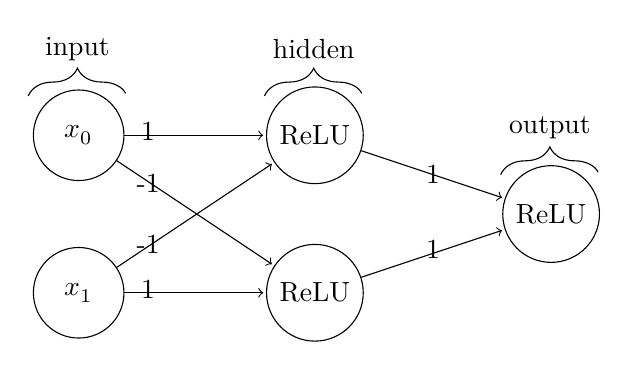
\begin{tikzpicture}[shorten >=1pt]
      \tikzstyle{unit}=[draw,shape=circle,minimum size=1.15cm]
      %\tikzstyle{hidden}=[draw,shape=circle,fill=black!25,minimum size=1.15cm]
      \tikzstyle{hidden}=[draw,shape=circle,minimum size=1.15cm]
   
      \node[unit](x1) at (0,2){$x_0$};
      \node[unit](x0) at (0,0){$x_1$};
   
      \node[unit](h1) at (3,2){ReLU};
      \node[unit](h0) at (3,0){ReLU};

      \node[unit](o1) at (6,1){ReLU};
   
      \draw[->] (x0) -- (h0) node [black,midway,xshift=-0.6cm,yshift=+0.05cm]{1};
      \draw[->] (x0) -- (h1)node [black,midway,xshift=-0.6cm,yshift=+0.4cm]{-1};
   
      \draw[->] (x1) -- (h0)node [black,midway,xshift=-0.6cm,yshift=-0.4cm]{-1};
      \draw[->] (x1) -- (h1)node [black,midway,xshift=-0.6cm,yshift=+0.05cm]{1};
   
      \draw[->] (h0) -- (o1)node [black,midway,yshift=+0.05cm]{1};
      \draw[->] (h1) -- (o1)node [black,midway]{1};
      
      \draw [decorate,decoration={brace,amplitude=10pt},xshift=-4pt,yshift=0pt] (-0.5,2.5) -- (0.75,2.5) node [black,midway,yshift=+0.6cm]{input};
      \draw [decorate,decoration={brace,amplitude=10pt},xshift=-4pt,yshift=0pt] (2.5,2.5) -- (3.75,2.5) node [black,midway,yshift=+0.6cm]{hidden};
      \draw [decorate,decoration={brace,amplitude=10pt},xshift=-4pt,yshift=0pt] (5.5,1.5) -- (6.75,1.5) node [black,midway,yshift=+0.6cm]{output};
    \end{tikzpicture}
    \caption{XOR network}
  \end{figure}
\item
  a. the output is (4, 0)

  b. the output is (2.5, 0)
\end{enumerate}

\end{document}
